%  A simple AAU report template.
%  2014-09-13 v. 1.1.0
%  Copyright 2010-2014 by Jesper Kjær Nielsen <jkn@es.aau.dk>
%
%  This is free software: you can redistribute it and/or modify
%  it under the terms of the GNU General Public License as published by
%  the Free Software Foundation, either version 3 of the License, or
%  (at your option) any later version.
%
%  This is distributed in the hope that it will be useful,
%  but WITHOUT ANY WARRANTY; without even the implied warranty of
%  MERCHANTABILITY or FITNESS FOR A PARTICULAR PURPOSE.  See the
%  GNU General Public License for more details.
%
%  You can find the GNU General Public License at <http://www.gnu.org/licenses/>.
%
\iflanguage{english}
{\pdfbookmark[0]{Frontpage}{label:frontpage}}%
{\pdfbookmark[0]{Forside}{label:forside}}%

\begin{titlepage}
  \addtolength{\hoffset}{0.5\evensidemargin-0.5\oddsidemargin} %set equal margins on the frontpage - remove this line if you want default margins
  \noindent%
  \begin{tabular}{@{}p{\textwidth}@{}}
    \toprule[2pt]
    \midrule
    \vspace{0.2cm}
    \begin{center}
    \huge{\textbf{
      \projectTitle% You can change the title in projectinfo.tex
    }}
    \end{center}
%    \begin{center}
%      \Large{
%        \projectSubtitle% insert your subtitle here
%      }
%    \end{center}
    \vspace{0.2cm}\\
    \midrule
    \toprule[2pt]
  \end{tabular}
  \vspace{2 cm}
  \begin{center}
    {\large
      \projectType%Insert document type (e.g., Project Report)
    }\\
    \vspace{0.2cm}
    {\Large
      \projectParticipants%Insert your group name or real names here 
\begin{figure}[H]
\centering
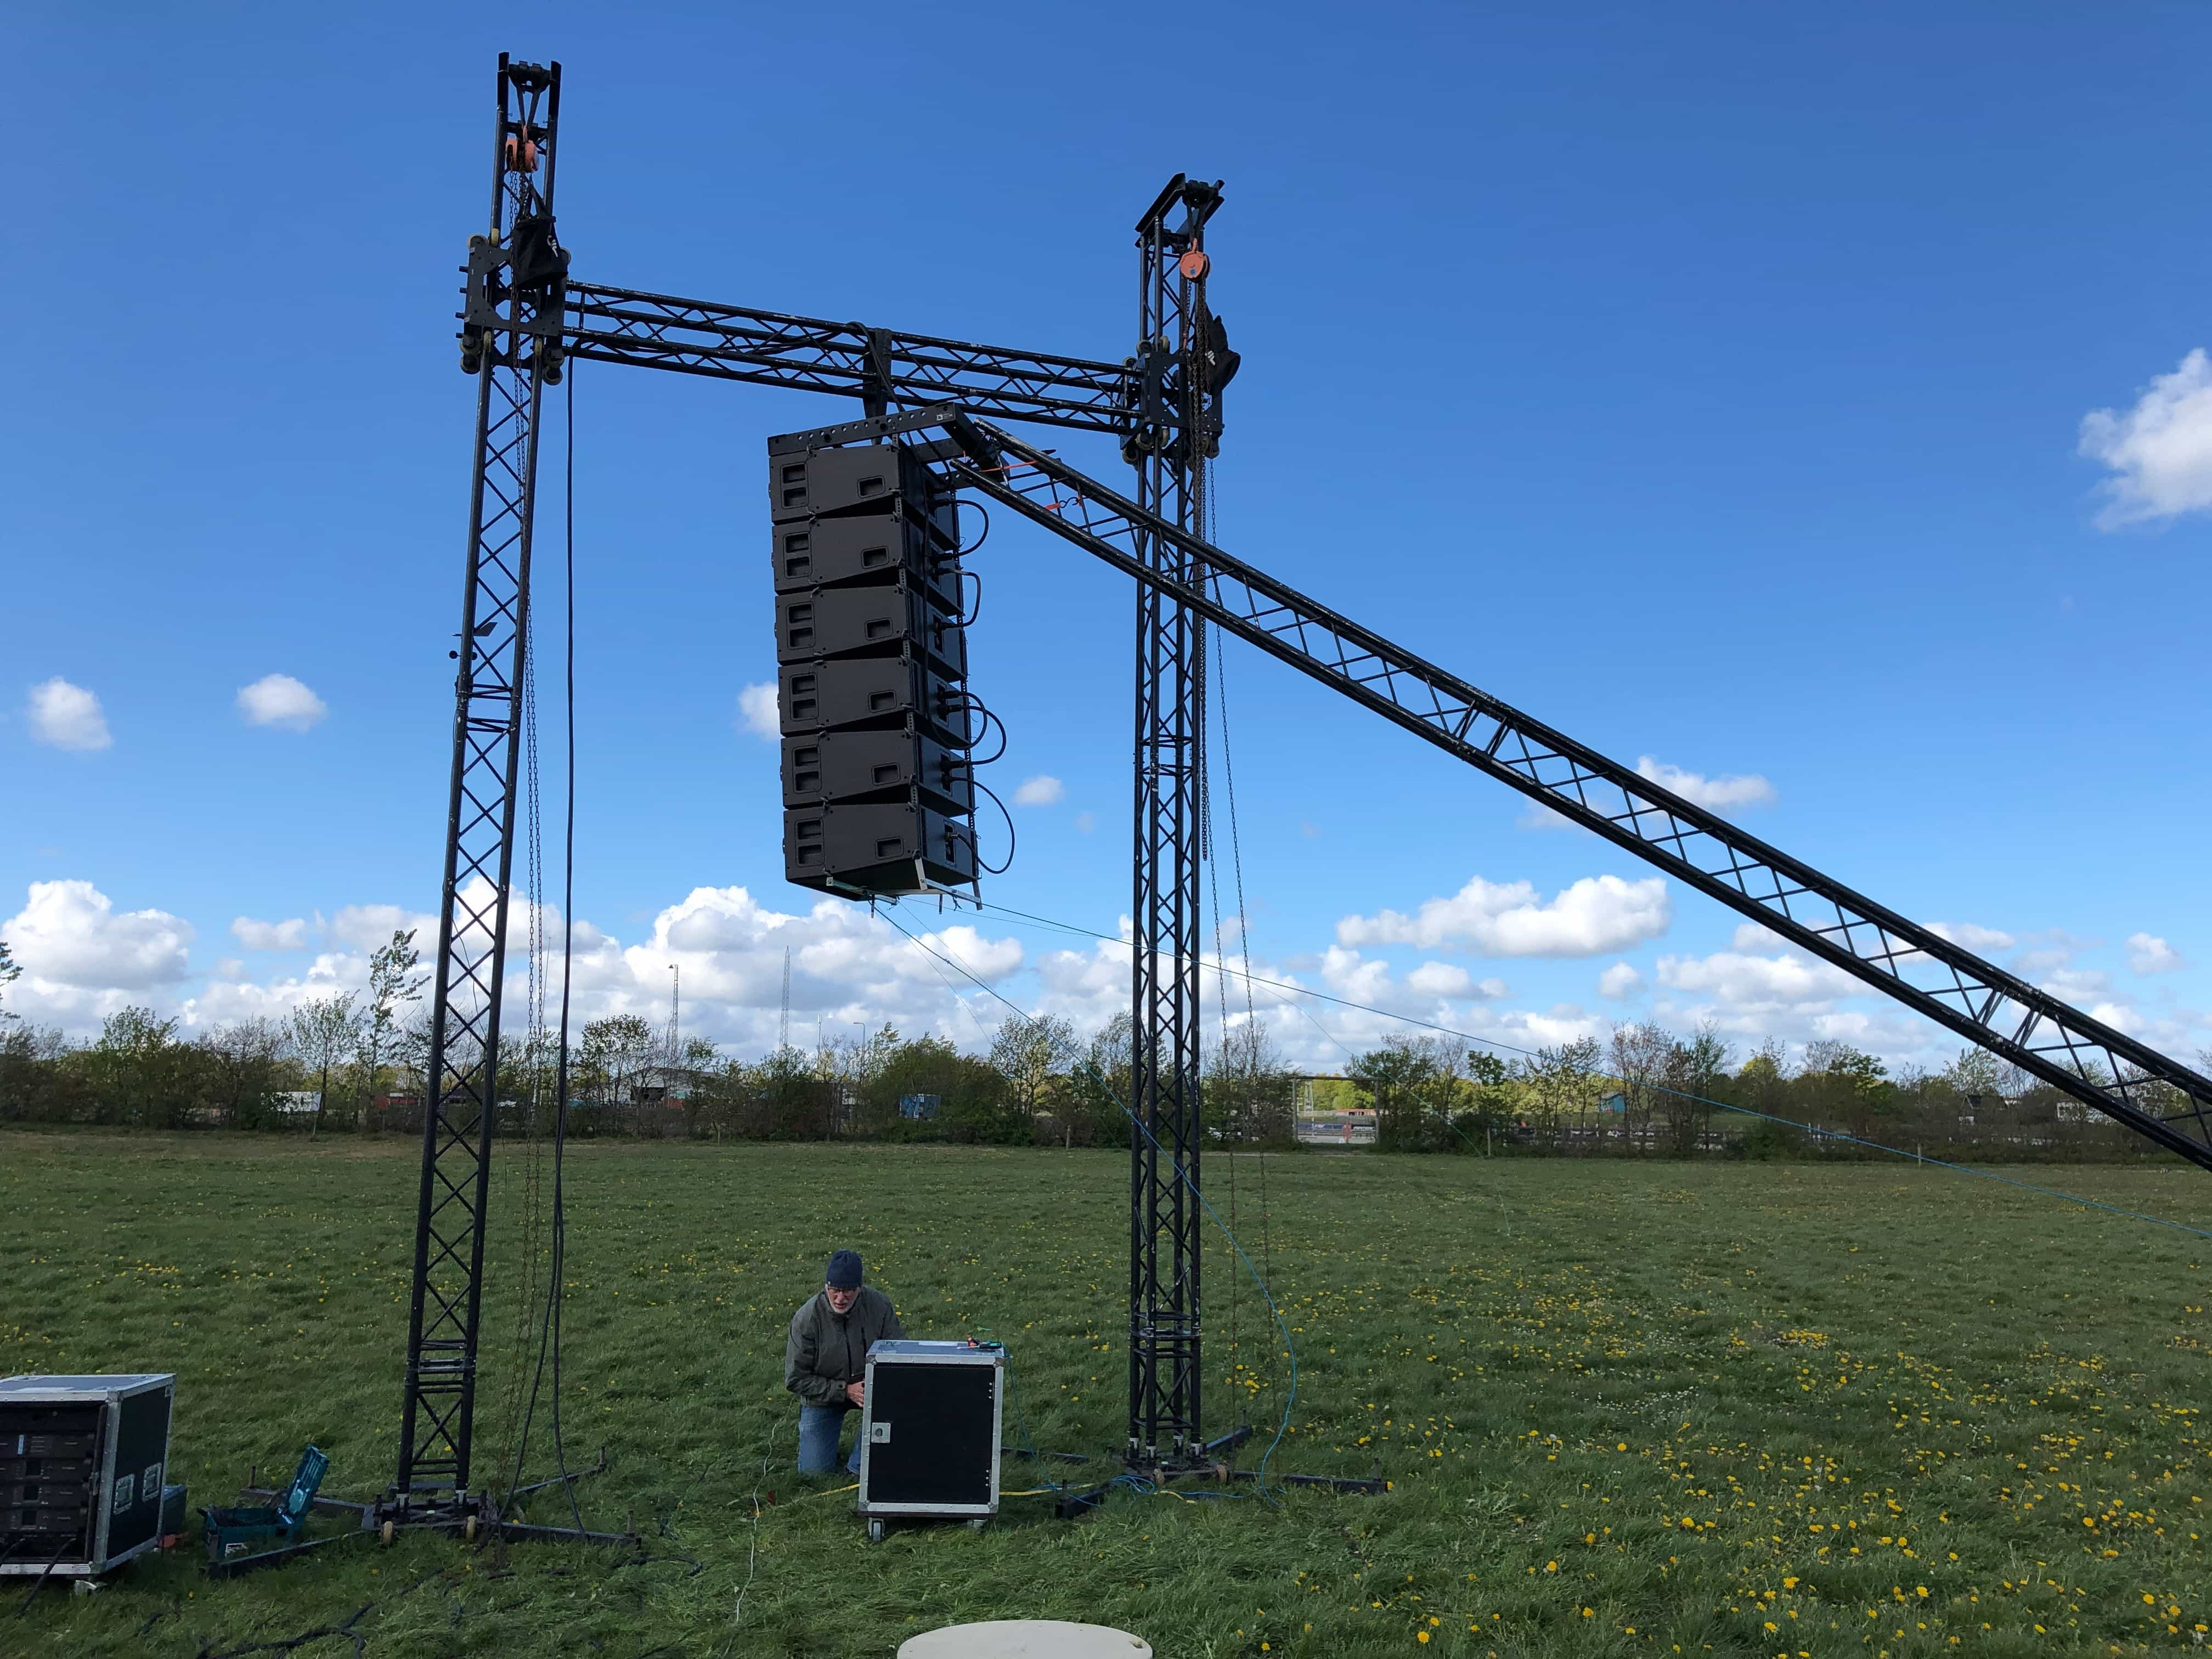
\includegraphics[width=1\textwidth]{IMG_0174}
\end{figure}
    }
  \end{center}
  \vfill
  \begin{center}
  \iflanguage{english}{Aalborg University}{Aalborg Universitet}\\
  \projectFaculty
  \end{center}
\end{titlepage}
\clearpage
